\chapter{Roadmap Methods for Motion Planning}
\label{chap:roadmaps}

The motion planning problem is a fundamental problem in robotics.
This chapter describes the motion planning problem,
and provides an overview of a well-studied class of algorithms called
roadmap methods.
We focus only on the parts that are relevant to this thesis;
for a more comprehensive treatment,
see LaValle \citep{lavalle2006planningbook}.

\section{The Motion Planning Problem}

The earliest examples considered were for a single rigid body.
The most fundamental form of the \emph{motion planning problem},
which is a generalization of the \emph{piano mover's problem},
entails x y and z.
Cites:
\citep{lozanoperezwedley1979collisionfree}.
Piano mover's problem
\citep{schwartzsharir1983pianomovers1}.
All about geometry, valid/invalid poses.
Find a solution, or determine that no solution exists.
Problems characterized by finding collision-free paths,
or proving that none exist.
Intimately related to the geometry of the body and of the obstacles.
Introduce feasibiliy / infeasibility.

Originally, for a rigid body
in a 2D or 3D workspace.
Various different specifications of types of obstacles (polygonal regions)
and types of bodies.

The generalization called the \emph{motion planning problem}
deals with configuration spaces.
Cite: \citep{lozanoperez1983cspace}.
We can deal with articulated mechanisms,
which we focus on in this thesis.
It is fundamental to robotics.
Problem also called FindPath.

Define $\mathcal{C}_{\ms{free}}$.
Compact sets.

A solution is called a path.

What are its properties?

\begin{itemize}
\item The space is continuous.
\item Solutions are continuous (and there are an infinite set of them).
\end{itemize}

\subsection{Optimal Motion Planning}

The optimal motion planning problem is a generalization which
includes a metric over solution paths.

\subsection{Further Generalizations}

There are other generalizations such as kinodynamic planning.
Here, a solution is commonly called a trajectory.
Optimal variants may have costs on the actions as well.
Intro: focus on configuration-space planning (not kinodynamic planning).

What about constraints? We won't deal with these much either.

\section{Motion Planning by Discretizing C-Space}

\subsection{Testing Validity of Motions}

Well, there are exact algorithms.
Exact methods in low-dimensional spaces.
The key point here is that these methods do not rely on discretization
of the configuration space.
But representing C-space obstacles is too hard.
(Cite for one approach: \citep{lozanoperez1983cspace}.)
Instead, we validate paths via lifting samples
into 3D space and testing them.
Relate to term ``sampling-based methods.''

Talk about committing to a resolution to test with,
which is what we do in this thesis.
Note that this is only an approximation.
You should pad your obstacles so you don't plan through wires.
But also link to C-space bubble stuff.

Define the path indicator function.

\subsection{Graphs in C-Space}

Due to the way we test paths for validity,
it is natural to explore algorithms which build larger paths
out of smaller ones.
We focus on algorithms that approximate C-space via graphs.
Talk about discretizing states.

There are other ways that don't discretize C-Space this way.
E.g. optimizataion approaches (CHOMP, TrajOpt) which require
stronger world descriptions (SDFs, convex obstacle decompositions).

The key point of this section is whether the algorithm commits to
a discretization a priori,
or whether the graph is built incrementally in response to the
distribution of valid or costly states.

\subsection{Resolution and Probabalistic Completeness}

Of course, the discretization is always just an approximation
of the actual C-space.
Hopefully, you can choose a discretization strategy that allows your
algorithm to have one or both of these forms of completeness.

\section{Obstacle-Insensitive Discretizations}

So we've decided to build graphs in C-space to answer motion planning
queries.
The next question is what should characterize our approach.

We focus on discretizations that are obstacle-insensitive.
Here's why.

\subsection{Obstacle Insensitive Approaches}

The most straightforward discretezation strategy.
Commit to a graph structure a priori.

Examples (we'll talk a lot more about this in the next section).
\begin{itemize}
\item Lattices (Graph search methods, A*, etc).
\item RGGs (PRMs, FMT* \citep{janson2015fmtstar},
   BIT* \citep{gammell2015bitstar}).
\item Halton graphs.
\end{itemize}

What about densification? (aka adaptive discretization)

\subsection{Obstacle Sensitive Approaches}

Many approaches build graphs incrementally in response to the
obstacle distribution.

RRT.

Visibility PRMs \citep{simeon2000visibilityprms}.

Smart sampling strategies.
Talk about sampling heuristics.
The original PRM.
Lots of other things.

Expansive spaces.
ESTs. Expansive spaces. \citep{hsu1997expansive}.

Usually, densification comes for free.

Probabalistic completeness.

\subsection{Conclusion}

Of course, lots of planners do both.
Often, use sensitivity for better performance,
and mix in some insensitivity for completeness properties.

Talk about adaptive discretization.

Bonus of obstacle insensitivity: caching, parallelization.
Central point: by staying obstacle-agnostic, it's easier to cache
things that apply across problem instances.

But what type of obstacle-insensitive discretezation strategy should
we use?

\section{Determinism vs. Probabalisticness}

OK, so we've committed to an obstacle-insensitive discretization
strategy.
What type of graph should we choose?

\begin{figure}
   \centering
   \includegraphics{build/roadmaps/gen/aagrid}
   \includegraphics{build/roadmaps/gen/rgg}
   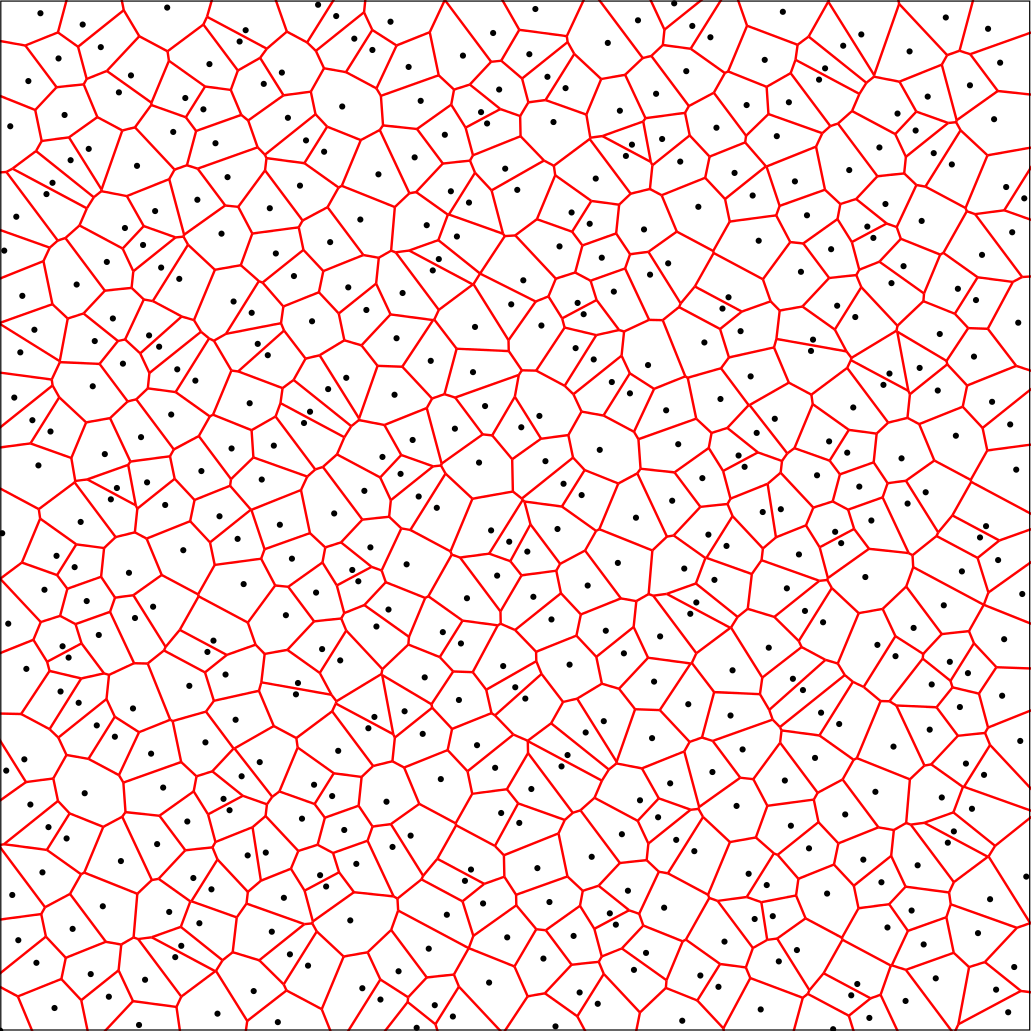
\includegraphics{build/roadmaps/gen/halton}
   \caption{Examples of roadmap types over the unit square
      (axis-aligned lattice, RGG, and Halton graphs).
      In this case, all roadmaps have a connection radius of 0.3.}
\end{figure}

Probabalistic vs. deterministic.
\citep{branicky2002detvsprobroadmaps}.
\citep{lavalle2002gridprms}.

\citep{janson2015deterministicsampling}.

Talk about probabalistic completeness and resolution completeness
\citep{cheng2004rescomplete}.

RRT* \citep{karaman2010rrtstar}.
Karaman/Frazzoli \citep{karaman2011samplingoptimal}.

RGGs.

Central point: densified roadmap strategy with good properties.

\begin{equation}
   \gamma^*_{\mathcal{C}}
      = 2 \left( \left[ 1 + \frac{1}{d} \right]
         \frac{\lambda_d(\mathcal{C})}{\zeta_d} \right)^{1/d}
\end{equation}

with $\lambda_d(\cdot)$ the Lebesgue measure of a $d$-dimensional
space.

Scaling radii:

\begin{equation}
   r_1(n) = \gamma_{\mathcal{C}} \left( \frac{\log(n)}{n} \right)^{1/d}
\end{equation}

\begin{equation}
   r_2(n) = \gamma_{\mathcal{C}} \left( \frac{\log(\log(n))}{n} \right)^{1/d}
\end{equation}

\begin{verbatim}
robot: HERB (n=10000)
radius log_n: 2.825833
radius loglog_n: 2.306115

robot: IRB4400 (n=10000)
radius log_n: 2.413850
radius loglog_n: 1.904293
\end{verbatim}

\subsection{Dispersion}

Deterministic sampling and dispersion:
\citep{janson2015deterministicsampling}.

\begin{figure}
   \centering
   \includegraphics{build/roadmaps-dispersion/dispersion}
   \caption{Dispersion plot.}
\end{figure}

\begin{figure}
   \centering
   \includegraphics{build/roadmaps-dispersion/dispersion-herb}
   \caption{HERB dispersion plot.}
\end{figure}

\begin{figure}
   \centering
   \includegraphics{build/roadmaps-dispersion/dispersion-irb4400}
   \caption{IRB4400 dispersion plot.}
\end{figure}

\subsection{Batch Size}

\begin{figure}
   \centering
   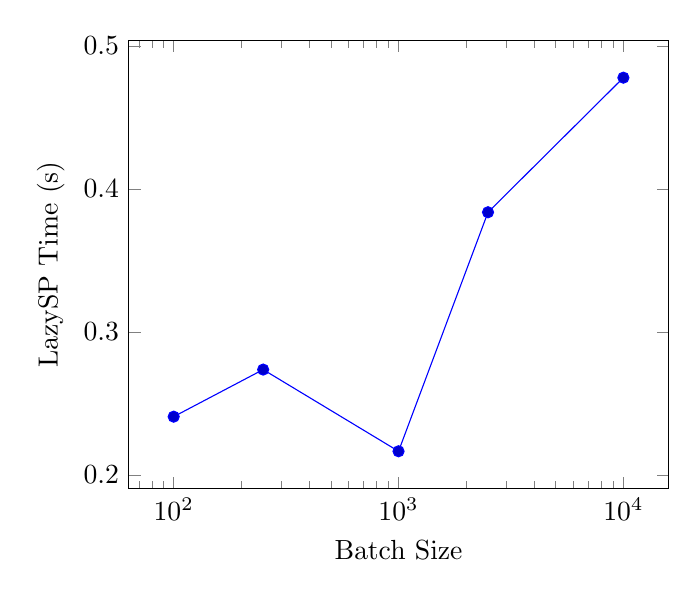
\begin{tikzpicture}
   \begin{axis}[
         xmode=log,
         xlabel={Batch Size},
         ylabel={LazySP Time (s)},
         xlabel near ticks,
         ylabel near ticks,
         ]
      \addplot coordinates {
         (100, 0.2407595708)
         (250, 0.27367886569999994)
         (1000, 0.2165730066)
         (2500, 0.3836524094)
         (10000, 0.47772694290000006)
      };
   \end{axis}
   \end{tikzpicture}
   \caption{Batch size. {\tt herbbin0}, seeds 1-10, gammafac=1, lambda=0.}
\end{figure}
